The receiver is basically a robot driven by the commands from the Discovery board, which communicates through the Bluetooth channel. The receiver is provided by an opportune object to take the data, ignore the eventual dirty characters, and execute what is required.

\subsection{Main parts}
The robot is divided in three main parts:
\begin{itemize}
	\item The serial communication: this is the section that is in charge of receiving and sending strings, encapsulating all the code within an object and, consequently, allowing changes and extensions;
	\item The Executer: this is the object that, given a command stored in a string, looks for a function able to execute it and, in positive case, runs it;
	\item The controller: this is the part performed by the Arduino \textit{loop} method and provides to invoke the serial communication methods, taking the commands strings and giving them to the executer.
\end{itemize}

\subsection{The serial communication}
\begin{figure}[h!]
	\centering
	\hspace*{-0.25 \textwidth}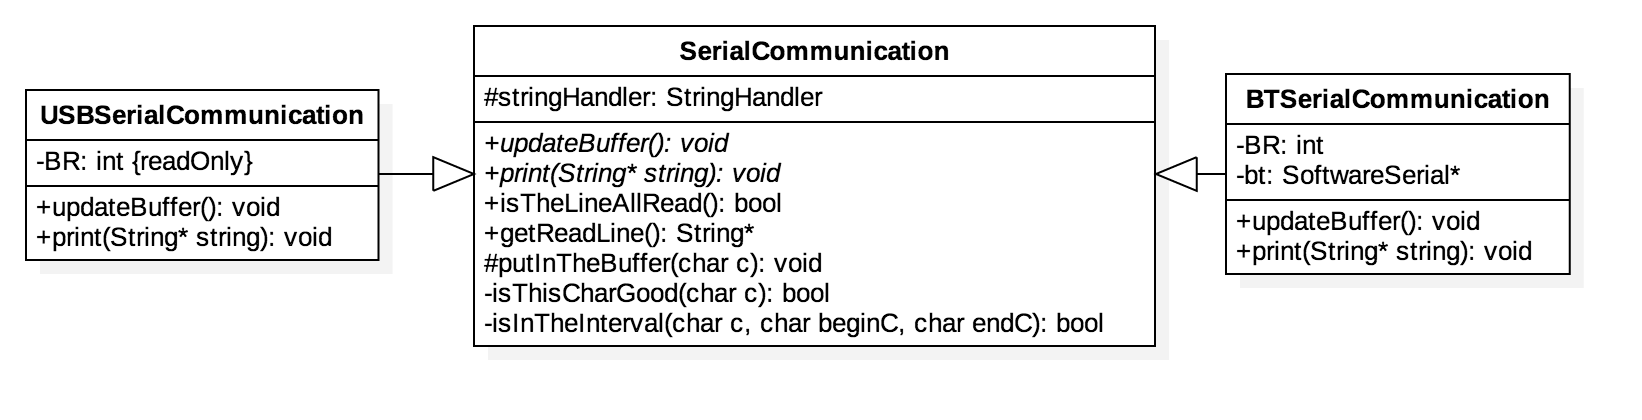
\includegraphics[width= 1.5\textwidth]
	{files/images/ArduinoConnection}
	\caption{The structure of the connection in the receiver.}
	\label{fig:connection}
\end{figure}
The \textit{SerialCommunication} class is a generic structure that takes the characters from a source and converts them in strings. Consequently, this class provides few important methods to improve and to organize this process, used independently by the source nature:
\begin{itemize}
	\item \textit{updateBuffer}: this method is used to take the available characters from the receiver buffer and put them in a temporary opportune storage object (\textit{StringHandler}). If there is no characters or a line is fully read, this method simply does nothing.
	\item \textit{isAllTheLineRead}: this methods returns true if a line is fully read, else it returns false.
	\item \textit{readLine}: this returns in a string all the read characters, independently if a line is fully received, and empties the buffer in \textit{StringHandler}.
	\item \textit{print}: this method prints the passed string on the connection channel, adding automatically the end line character.
\end{itemize}

\subsubsection{\textit{StringHandler}}
All the received characters are temporary stored in an apposite data structure, called \textit{StringHandler}. This class offers some methods to manipulate these characters, allowing to know if a string is fully received and, eventually, withdraw it. It's not necessary that the string is fully received to transform all the received character in a string. After the withdraw method invocation, the object resets itself.

\subsubsection{\textit{SerialCommunication} extensions}
In the Figure \ref{fig:connection}, in particular in the parent class, two methods are indicate as virtual, since their implementation depends by the connection type used. Consequently, the \textit{SerialCommunication} class was extended by \textit{BTSerialCommunication} and by \textit{USBSerialCommunication}, which implement these two methods, according to their specification and using proper attributes to perform these actions.\\
In the communication, the class \textit{USBSerialCommunication} and the \textit{print} method of \textit{BTSerialCommunication} are implemented but never used. They were added for debug features and for future expansion, made easier by this organization.

\subsection{The Executer}
The \textit{Executer} interprets the received commands by the connection. A command is a string that has, as first character, a proper name and, subsequently, some parameters for that specific command. Its name is used to get, with a constant time through an Hash map, the method to invoke for executing that specific command. This class exposes only a method, the one invoked passing the string as parameter and that researches and executes the opportune function.\\*
This structure allows to extends the robot with future modules, without changing this object but just adding the new function pointers to the map.\\*

\subsubsection{The used Hash map}
The quoted Hash map is not a class from the library but a proper class implemented in this code. It is not a perfect Hash function since it uses the module operation to compute the indexes but this choice was made to avoid useless computational time wastes. It is however possible change it since it is fully encapsulated in a module.\\

\subsubsection{The used commands}
This robot uses the following commands:
???

\subsection{The circuit}
\begin{figure}[h!]
	\centering
	\hspace*{-0.05 \textwidth}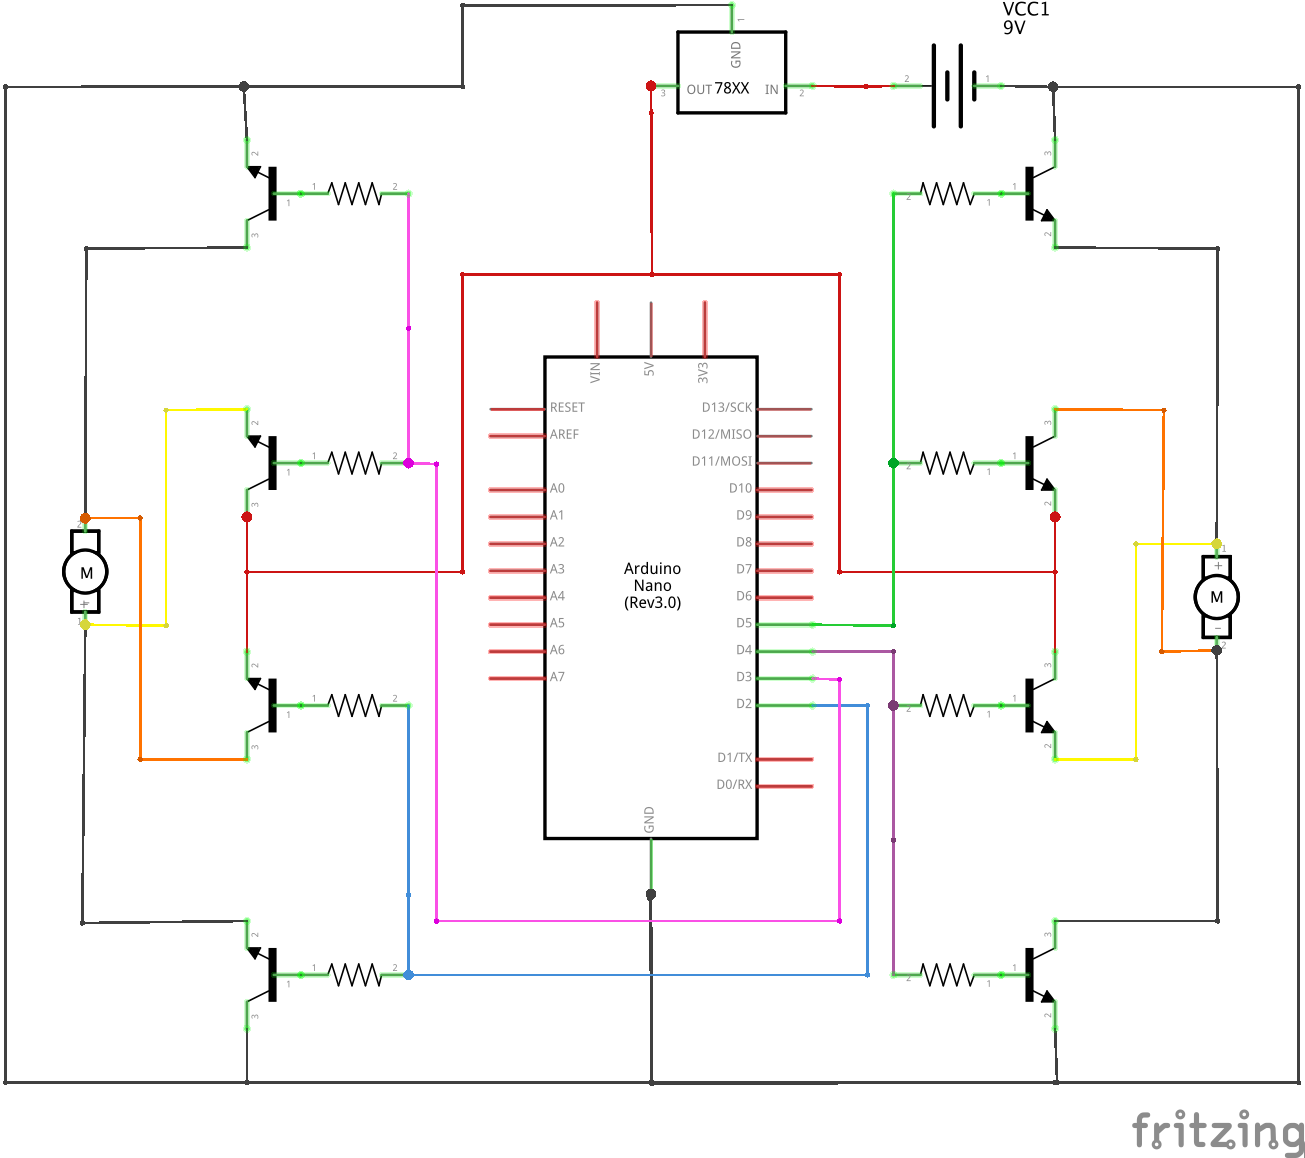
\includegraphics[width= 1.1\textwidth]
	{files/images/ReceiverScheme}
	\caption{The motors circuit scheme of the robot.}
\end{figure}
For this robot, is necessary that both the motors rotate in two different directions, consequently, it is implemented two basic \textit{H bridges} to perform this purpose. To avoid the use of inverters, it is necessary uses two pins for each motor direction and so eight Arduino pins are used to handle the movements.\\
In other two pins, the Bluethooth module HC05 text and read pins are connected, despite it isn't shown in the circuit scheme. Also the LEDs and the eventual buzzer aren't shown.